%% State Space Modelling of Dynamic Systems
%% Lecture 2: Transforms and Time Responses of State-Space Models
\def\FileDate{99/10/06}
\def\FileVersion{1.2}
% ----------------------------------------------------------------
% Notes pages *********************************************************
% ----------------------------------------------------------------

\begin{slide}
   \heading{Transforms and Time Responses for SS Models}
   \begin{itemize}
   	\item Laplace Transform of State Space Models
   	\item Time Responses for State Space Models
   	\item Problems
   \end{itemize}
\end{slide}

\section*{Transforms of State Space Models} % (fold)
\label{sec:transforms_of_state_space_models}

The Laplace transform can be used to convert a differential equation
into a transfer function. It can also be used to convert a state space
model into a transfer function. In this lecture we demonstrate how
this is done and we give an example.

\ifslidesonly
\begin{slide}
  \heading{Laplace transform of a vector of functions}
  
\begin{center}
	\resizebox{200pt}{!}{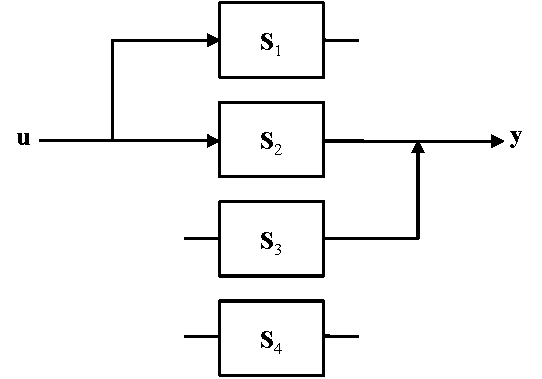
\includegraphics{pictures/partitioning.pdf}}
\end{center}
\endinput

%%% Local Variables: 
%%% mode: latex
%%% TeX-master: "notes"
%%% End:
\end{slide}
\fi

\begin{center}
	\resizebox{200pt}{!}{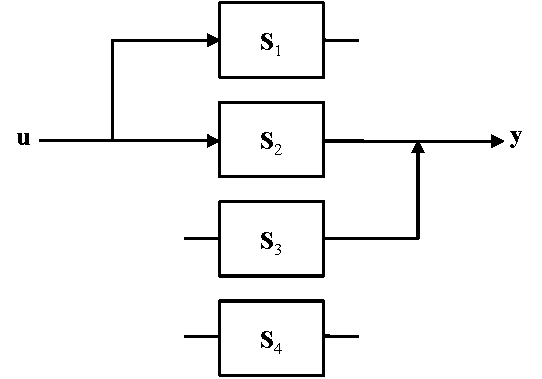
\includegraphics{pictures/partitioning.pdf}}
\end{center}
\endinput

%%% Local Variables: 
%%% mode: latex
%%% TeX-master: "notes"
%%% End:

\ifslidesonly
\begin{slide}
  \heading{Laplace transform of a vector of functions (cont)}
  If we write down the equations for the elements we get:
\begin{eqnarray}
  \frac{dv_{31}}{dt} &=& \frac{1}{C}\ i_2 \label{eq:l13e1}\\
  \frac{di_{i}}{dt} &=& \frac{1}{L}\ v_{32} \label{eq:l13e2}\\
  v_{21} &=& R\ i_1 \label{eq:l13e3}
\end{eqnarray}
The ``compatability'' and ``continuity'' equations are
\begin{eqnarray}
  u &=& i_1 + i_2 \label{eq:l13e4}\\
  v_{31} &=& v_{32} + v_{21} \label{eq:l13e5}
\end{eqnarray}

\endinput
%%% Local Variables: 
%%% mode: latex
%%% TeX-master: "notes"
%%% End: 

\end{slide}
\fi
If we write down the equations for the elements we get:
\begin{eqnarray}
  \frac{dv_{31}}{dt} &=& \frac{1}{C}\ i_2 \label{eq:l13e1}\\
  \frac{di_{i}}{dt} &=& \frac{1}{L}\ v_{32} \label{eq:l13e2}\\
  v_{21} &=& R\ i_1 \label{eq:l13e3}
\end{eqnarray}
The ``compatability'' and ``continuity'' equations are
\begin{eqnarray}
  u &=& i_1 + i_2 \label{eq:l13e4}\\
  v_{31} &=& v_{32} + v_{21} \label{eq:l13e5}
\end{eqnarray}

\endinput
%%% Local Variables: 
%%% mode: latex
%%% TeX-master: "notes"
%%% End: 


\ifslidesonly
\begin{slide}
  \heading{Example}
  Given the transformation $\mathbf{T}^{-1}\mathbf{AT}=\mathbf{\Lambda}$:
\begin{eqnarray*}
	\mathbf{A}t & = & (\mathbf{T\Lambda T}^{-1}) t \\
	\mathbf{A}^nt^n & = & (\mathbf{T\Lambda T}^{-1})(\mathbf{T\Lambda T}^{-1})\ldots(\mathbf{T\Lambda T}^{-1})t^n \\
	                & = & \mathbf{T\Lambda T}^{-1}\mathbf{T\Lambda T}^{-1}\ldots\mathbf{T\Lambda T}^{-1}t^n \\
	\mathbf{A}^nt^n & = & \mathbf{T\Lambda}\mathbf{I}\mathbf{\Lambda I}\ldots\mathbf{I\Lambda T}^{-1}t^n \\
	\               & = & \mathbf{T\Lambda}^n\mathbf{T}^{-1}t^n \\
\end{eqnarray*}
\endinput

%%% Local Variables: 
%%% mode: latex
%%% TeX-master: "notes"
%%% End:
\end{slide}
\fi
Given the transformation $\mathbf{T}^{-1}\mathbf{AT}=\mathbf{\Lambda}$:
\begin{eqnarray*}
	\mathbf{A}t & = & (\mathbf{T\Lambda T}^{-1}) t \\
	\mathbf{A}^nt^n & = & (\mathbf{T\Lambda T}^{-1})(\mathbf{T\Lambda T}^{-1})\ldots(\mathbf{T\Lambda T}^{-1})t^n \\
	                & = & \mathbf{T\Lambda T}^{-1}\mathbf{T\Lambda T}^{-1}\ldots\mathbf{T\Lambda T}^{-1}t^n \\
	\mathbf{A}^nt^n & = & \mathbf{T\Lambda}\mathbf{I}\mathbf{\Lambda I}\ldots\mathbf{I\Lambda T}^{-1}t^n \\
	\               & = & \mathbf{T\Lambda}^n\mathbf{T}^{-1}t^n \\
\end{eqnarray*}
\endinput

%%% Local Variables: 
%%% mode: latex
%%% TeX-master: "notes"
%%% End:
\ifslidesonly
  \begin{slide}
    \heading{Transform of state equations}
    The matrix function becomes:
\begin{eqnarray*}
	f(\mathbf{A}t) & = & f_0\mathbf{TIT}^{-1} + f_1\mathbf{T\Lambda T}^{-1}t + f_2\mathbf{T\Lambda}^2\mathbf{T}^{-1}t^2 + \cdots + f_n\mathbf{T\Lambda}^n\mathbf{T}^{-1}t^n + \cdots \\
	f(\mathbf{A}t) & = & \mathbf{T}\left(f_0\mathbf{I} + f_1\mathbf{\Lambda}t + f_2\mathbf{\Lambda}^2t^2 + \cdots + f_n\mathbf{\Lambda}^nt^n + \cdots \right)\mathbf{T}^{-1}\\
	               & = & \mathbf{T}f(\mathbf{\Lambda}t)\mathbf{T}^{-1}
\end{eqnarray*}
 
The term inside the brackets on the rhs is a diagonal matrix and the $i^\mathrm{th}$ diagonal element is:
\[
f_0+f_1\lambda_it + f_2\lambda_i^2t^2 + \cdots + f_n\lambda_i^nt^ + \cdots
\]
From the Taylor series this must be $f(\lambda_i t)$:
\[
f(\mathbf{A} t)=\mathbf{T} f(\mathbf{\Lambda} t) \mathbf{T}^{-1}
\]   
where $f(\mathbf{\Lambda} t)=\mathrm{diag}\left(f(\lambda_i t)\right)$.

\endinput

%%% Local Variables: 
%%% mode: latex
%%% TeX-master: "notes"
%%% End:
  \end{slide}
\fi
The matrix function becomes:
\begin{eqnarray*}
	f(\mathbf{A}t) & = & f_0\mathbf{TIT}^{-1} + f_1\mathbf{T\Lambda T}^{-1}t + f_2\mathbf{T\Lambda}^2\mathbf{T}^{-1}t^2 + \cdots + f_n\mathbf{T\Lambda}^n\mathbf{T}^{-1}t^n + \cdots \\
	f(\mathbf{A}t) & = & \mathbf{T}\left(f_0\mathbf{I} + f_1\mathbf{\Lambda}t + f_2\mathbf{\Lambda}^2t^2 + \cdots + f_n\mathbf{\Lambda}^nt^n + \cdots \right)\mathbf{T}^{-1}\\
	               & = & \mathbf{T}f(\mathbf{\Lambda}t)\mathbf{T}^{-1}
\end{eqnarray*}
 
The term inside the brackets on the rhs is a diagonal matrix and the $i^\mathrm{th}$ diagonal element is:
\[
f_0+f_1\lambda_it + f_2\lambda_i^2t^2 + \cdots + f_n\lambda_i^nt^ + \cdots
\]
From the Taylor series this must be $f(\lambda_i t)$:
\[
f(\mathbf{A} t)=\mathbf{T} f(\mathbf{\Lambda} t) \mathbf{T}^{-1}
\]   
where $f(\mathbf{\Lambda} t)=\mathrm{diag}\left(f(\lambda_i t)\right)$.

\endinput

%%% Local Variables: 
%%% mode: latex
%%% TeX-master: "notes"
%%% End:

For the system in the example the state vector is defined as
$\mathbf{x}=[v_{31}, i_1]^{T}$, the input current is $u$, and the output
variables are all the currents and voltages in the circuit
$\mathbf{y}=[v_{31}, i_1, v_{32}, v_{21}, i_2]^{T}$. The transformed
state space model is therefore that shown in
\sref{slide:slide-l2eg1}.
\begin{slide}\label{slide:slide-l2eg1}
\heading{Transformed State-Equations for Example 1 from L12}
\begin{eqnarray*} s\left[\begin{array}{c}
  V_{31} \\
  I_1
\end{array}\right]-\left[\begin{array}{c}
  v_{31}(0) \\
  i_1(0)
\end{array}\right]&=&\left[\begin{array}{cc}
  0 & -1/C \\
  1/L & -R/L
\end{array}\right]\left[\begin{array}{c}
  V_{31} \\
  I_1
\end{array}\right]+\left[\begin{array}{c}
  1/C \\
  0
\end{array}\right]\left[U\right]\\
\left[\begin{array}{c}
  V_{31} \\
  I_1 \\
  V_{32} \\
  V_{21} \\
  I_{2}
\end{array}\right]&=&\left[\begin{array}{cc}
  1 & 0 \\
  0 & 1 \\
  1 & -R \\
  0 & R \\
  0 & -1
\end{array}\right]\left[\begin{array}{c}
  V_{31} \\
  I_1
\end{array}\right]+\left[\begin{array}{c}
  0 \\
  0 \\
  0 \\
  0 \\
  1
\end{array}\right]\left[U\right].
\end{eqnarray*}
\end{slide}

\ifslidesonly
\begin{slide}
\heading{Transfer function from state space models (1)}
The vector $[v_{31}, i_{1}]^T$ is called the ``\emph{state
vector}.'' Its elements are state variables.
\endinput
%%% Local Variables: 
%%% mode: latex
%%% TeX-master: "notes"
%%% End: 

\end{slide}\fiThe vector $[v_{31}, i_{1}]^T$ is called the ``\emph{state
vector}.'' Its elements are state variables.
\endinput
%%% Local Variables: 
%%% mode: latex
%%% TeX-master: "notes"
%%% End: 

\ifslidesonly
\begin{slide}\heading{Transfer function from state space models (2)}
From previous work the error dynamics are:
\[
\dot{\mathbf{e}} = (\mathbf{A}-\mathbf{LC})\mathbf{e}
\]
Therefore the dynamics of the combined system is:
\[\left[ {\begin{array}{*{20}c}
   {\dot{\mathbf{x}}}  \\
   {\dot{\mathbf{e}}ß}  \\
\end{array}} \right] = \left[ {\begin{array}{*{20}c}
   {\left( {{\bf{A}} - {\bf{BK}}} \right)} & {{\bf{BK}}}  \\
   {\bf{0}} & {\left( {{\bf{A}} - {\bf{LC}}} \right)}  \\
\end{array}} \right]\left[ {\begin{array}{*{20}c}
   {\bf{x}}  \\
   {\bf{e}}  \\
\end{array}} \right] + \left[ {\begin{array}{*{20}c}
   {\bf{B}}  \\
   {\bf{0}}  \\
\end{array}} \right]r
\]
\endinput

%%% Local Variables: 
%%% mode: latex
%%% TeX-master: "notes"
%%% End:
\end{slide}\fiFrom previous work the error dynamics are:
\[
\dot{\mathbf{e}} = (\mathbf{A}-\mathbf{LC})\mathbf{e}
\]
Therefore the dynamics of the combined system is:
\[\left[ {\begin{array}{*{20}c}
   {\dot{\mathbf{x}}}  \\
   {\dot{\mathbf{e}}ß}  \\
\end{array}} \right] = \left[ {\begin{array}{*{20}c}
   {\left( {{\bf{A}} - {\bf{BK}}} \right)} & {{\bf{BK}}}  \\
   {\bf{0}} & {\left( {{\bf{A}} - {\bf{LC}}} \right)}  \\
\end{array}} \right]\left[ {\begin{array}{*{20}c}
   {\bf{x}}  \\
   {\bf{e}}  \\
\end{array}} \right] + \left[ {\begin{array}{*{20}c}
   {\bf{B}}  \\
   {\bf{0}}  \\
\end{array}} \right]r
\]
\endinput

%%% Local Variables: 
%%% mode: latex
%%% TeX-master: "notes"
%%% End:
\ifslidesonly
\begin{slide}\heading{Transfer function from state space models (3)}
When the initial conditions of the state-variables are all zero,
this reduces to the transfer matrix model
\begin{equation}\label{eqn:transfer-function}
  \mathbf{Y}=\left[\mathbf{C}\left[s\mathbf{I}-\mathbf{A}\right]^{-1}\mathbf{B}+\mathbf{D}\right]\mathbf{U}
\end{equation}

\endinput

%%% Local Variables: 
%%% mode: latex
%%% TeX-master: "notes"
%%% End: 

\end{slide}\fiWhen the initial conditions of the state-variables are all zero,
this reduces to the transfer matrix model
\begin{equation}\label{eqn:transfer-function}
  \mathbf{Y}=\left[\mathbf{C}\left[s\mathbf{I}-\mathbf{A}\right]^{-1}\mathbf{B}+\mathbf{D}\right]\mathbf{U}
\end{equation}

\endinput

%%% Local Variables: 
%%% mode: latex
%%% TeX-master: "notes"
%%% End: 

\ifslidesonly
\begin{slide}\heading{Transfer function from state space models (4)}
When the observer canonical form is not used, then the design of the observer is more difficult. Ackermann's formula can be adapted as follows:
% MathType!MTEF!2!1!+-
% faaagaart1ev2aaaKnaaaaWenf2ys9wBH5garuavP1wzZbqedmvETj
% 2BSbqefm0B1jxALjharqqtubsr4rNCHbGeaGqiVu0Je9sqqrpepC0x
% bbL8FesqqrFfpeea0xe9Lq-Jc9vqaqpepm0xbba9pwe9Q8fs0-yqaq
% pepae9pg0FirpepeKkFr0xfr-xfr-xb9Gqpi0dc9adbaqaaeGaciGa
% aiaabeqaamaabaabaaGcbaGaaCitamaaCaaaleqabaGaamivaaaaki
% abg2da9maadmaabaqbamqabeabaaaabaGaaGimaaqaaiablAcilbqa
% aiaaicdaaeaacaaIXaaaaaGaay5waiaaw2faaiaad+eadaahaaWcbe
% qaaiabgkHiTiaaigdaaaGccqaHXoqydaWgaaWcbaGaam4yaaqabaGc
% caGGOaGaaCyqamaaCaaaleqabaGaamivaaaakiaacMcaaaa!3EF6!
\[
{\bf{L}}^T  = \left[ {\begin{array}{*{20}c}
   0 &  \ldots  & 0 & 1  \\
\end{array}} \right]\mathcal{O}^{ - 1} \alpha _e ({\bf{A}}^T )
\]
$\mathcal{O}$ is the observability matrix:
\[
\mathcal{O}=[\mathbf{C}^T\vdots\mathbf{A}^T\mathbf{C}^T\vdots\cdots\vdots(\mathbf{A}^T)^{n-1}\mathbf{C}^T]
\]
and if $\alpha_e(s)=s^n + \alpha_1s^{n-1}+\cdots+\alpha_n$ then \[\alpha_e(\mathbf{A}^T)=(\mathbf{A}^T)^n + \alpha_1(\mathbf{A}^T)^{n-1}+\cdots+\mathbf{I}\alpha_n.\]
 

Notice that if the system is unobservable, then the matrix inverse $\mathcal{O}^{-1}$ does not exist and we cannot design an observer for this system.


 
 

\endinput

%%% Local Variables: 
%%% mode: latex
%%% TeX-master: "notes"
%%% End:\end{slide}\fiWhen the observer canonical form is not used, then the design of the observer is more difficult. Ackermann's formula can be adapted as follows:
% MathType!MTEF!2!1!+-
% faaagaart1ev2aaaKnaaaaWenf2ys9wBH5garuavP1wzZbqedmvETj
% 2BSbqefm0B1jxALjharqqtubsr4rNCHbGeaGqiVu0Je9sqqrpepC0x
% bbL8FesqqrFfpeea0xe9Lq-Jc9vqaqpepm0xbba9pwe9Q8fs0-yqaq
% pepae9pg0FirpepeKkFr0xfr-xfr-xb9Gqpi0dc9adbaqaaeGaciGa
% aiaabeqaamaabaabaaGcbaGaaCitamaaCaaaleqabaGaamivaaaaki
% abg2da9maadmaabaqbamqabeabaaaabaGaaGimaaqaaiablAcilbqa
% aiaaicdaaeaacaaIXaaaaaGaay5waiaaw2faaiaad+eadaahaaWcbe
% qaaiabgkHiTiaaigdaaaGccqaHXoqydaWgaaWcbaGaam4yaaqabaGc
% caGGOaGaaCyqamaaCaaaleqabaGaamivaaaakiaacMcaaaa!3EF6!
\[
{\bf{L}}^T  = \left[ {\begin{array}{*{20}c}
   0 &  \ldots  & 0 & 1  \\
\end{array}} \right]\mathcal{O}^{ - 1} \alpha _e ({\bf{A}}^T )
\]
$\mathcal{O}$ is the observability matrix:
\[
\mathcal{O}=[\mathbf{C}^T\vdots\mathbf{A}^T\mathbf{C}^T\vdots\cdots\vdots(\mathbf{A}^T)^{n-1}\mathbf{C}^T]
\]
and if $\alpha_e(s)=s^n + \alpha_1s^{n-1}+\cdots+\alpha_n$ then \[\alpha_e(\mathbf{A}^T)=(\mathbf{A}^T)^n + \alpha_1(\mathbf{A}^T)^{n-1}+\cdots+\mathbf{I}\alpha_n.\]
 

Notice that if the system is unobservable, then the matrix inverse $\mathcal{O}^{-1}$ does not exist and we cannot design an observer for this system.


 
 

\endinput

%%% Local Variables: 
%%% mode: latex
%%% TeX-master: "notes"
%%% End:
\ifslidesonly
\begin{slide}\heading{The Resolvant Matrix}
\begin{itemize}
	\item Rule of thumb: observer poles can be faster than the controller poles (i.e. further from the origin) by a factor of 2 to 6. This makes the effect of the observer dynamics short-term and the overall response is dominated by the controller poles.
	\item If noise/disturbance is present this has an effect on the choice:
	\begin{description}
		\item[Process noise $w$:] $d\mathbf{x}/dt=\mathbf{Ax}+\mathbf{B}u+\mathbf{B}_1 w$
		\item[Sensor noise $v$:]  $y = \mathbf{C}x+v$
		\item[Observer:] $d\hat{\mathbf{x}}=\mathbf{A}\hat{\mathbf{x}}+\mathbf{B}u+\mathbf{L}(y-\mathbf{C}\hat{\mathbf{x}})$
		\item[Error $\mathbf{e}=\mathbf{x}-\hat{\mathbf{x}}$:] $d\mathbf{e}/dt=(\mathbf{A}-\mathbf{LC})\mathbf{e}+\mathbf{B}_1 w - \mathbf{L}v.$
	\end{description}
\end{itemize}

\endinput

%%% Local Variables: 
%%% mode: latex
%%% TeX-master: "notes"
%%% End:\end{slide}\fi\begin{itemize}
	\item Rule of thumb: observer poles can be faster than the controller poles (i.e. further from the origin) by a factor of 2 to 6. This makes the effect of the observer dynamics short-term and the overall response is dominated by the controller poles.
	\item If noise/disturbance is present this has an effect on the choice:
	\begin{description}
		\item[Process noise $w$:] $d\mathbf{x}/dt=\mathbf{Ax}+\mathbf{B}u+\mathbf{B}_1 w$
		\item[Sensor noise $v$:]  $y = \mathbf{C}x+v$
		\item[Observer:] $d\hat{\mathbf{x}}=\mathbf{A}\hat{\mathbf{x}}+\mathbf{B}u+\mathbf{L}(y-\mathbf{C}\hat{\mathbf{x}})$
		\item[Error $\mathbf{e}=\mathbf{x}-\hat{\mathbf{x}}$:] $d\mathbf{e}/dt=(\mathbf{A}-\mathbf{LC})\mathbf{e}+\mathbf{B}_1 w - \mathbf{L}v.$
	\end{description}
\end{itemize}

\endinput

%%% Local Variables: 
%%% mode: latex
%%% TeX-master: "notes"
%%% End:

For the system in the example, the resolvent matrix is developed
in \sref{slide:l2eg2}.
\begin{slide}\label{slide:l2eg2}
\heading{Resolvent matrix for the example}
\begin{eqnarray*}
\mathbf{A}&=&\left[\begin{array}{cc}
  0 & -1/C \\
  1/L & -R/L
\end{array}\right] \\
s\mathbf{I}-\mathbf{A}&=&\left[
\begin{array}{cc}
  s & 0 \\
  0 & s
\end{array}
\right] - \left[
\begin{array}{cc}
  0 & -1/C \\
  1/L & -R/L
\end{array}
\right] = \left[
\begin{array}{cc}
  s & +1/C \\
  -1/L & s+R/L
\end{array}\right] \\
\left[s\mathbf{I}-\mathbf{A}\right]^{-1}&=&\frac{
\left[\begin{array}{cc}
  s+R/L & -1/C \\
  +1/L & s
\end{array} \right]
}{s(s+R/L)+1/(LC)}=\frac{\left[\begin{array}{cc}
  s+R/L & -1/C \\
  +1/L & s
\end{array} \right]}{s^2 + (R/L)s + 1/(LC) }
\end{eqnarray*}
\end{slide}

When $\left[s\mathbf{I}-\mathbf{A}\right]^{-1}$ has been obtained,
then the system transfer function is easily obtained through
$\mathbf{C}\left[s\mathbf{I}-\mathbf{A}\right]^{-1}\mathbf{B}+\mathbf{D}$.
For the system in the example, when all outputs are measured, the
system transfer matrix is that shown in \sref{slide:l2eg3}.

\begin{slide}\label{slide:l2eg3}
\heading{Transfer matrix for example}
\begin{eqnarray*}
\left[\begin{array}{cc}
  1 & 0 \\
  0 & 1 \\
  1 & -R \\
  0 & R \\
  0 & -1
\end{array}\right]
\left\{\frac{\left[
\begin{array}{cc}
  s+R/L & -1/C \\
 +1/L & s
\end{array}\right]}{s^2 + (R/L)s +1/(LC)}\right\}
\left[\begin{array}{c}
  1/C \\
  0
\end{array}\right]
 &+& \left[\begin{array}{c}
  0 \\
  0 \\
  0 \\
  0 \\
  1
\end{array} \right]\\
= \left[\begin{array}{cc}
  1 & 0 \\
  0 & 1 \\
  1 & -R \\
  0 & R \\
  0 & -1
\end{array}\right]
\left\{\frac{\left[
\begin{array}{c}
  (1/C)s+R/(LC)  \\
 +1/(LC)
\end{array}\right]}{s^2 + (R/L)s +1/(LC)}\right\}
 &+& \left[\begin{array}{c}
  0 \\
  0 \\
  0 \\
  0 \\
  1
\end{array} \right]\\
\end{eqnarray*}
\end{slide}
\begin{slide}
\heading{Transfer matrix for example (completed)}
\begin{eqnarray*} &=& \frac{1}{s^2 + (R/L)s
+1/(LC)}\left[\begin{array}{c}
  (1/C)s+R/(LC) \\
  1/(LC) \\
  (1/C)s \\
  R/(LC) \\
  -1/(LC)
\end{array}\right] + \left[\begin{array}{c}
  0 \\
  0 \\
  0 \\
  0 \\
  1
\end{array} \right]\\
&=& \left[\begin{array}{c}
  \frac{(1/C)s+R/(LC)}{s^2 + (R/L)s
+1/(LC)} \\
  \frac{1/(LC)}{s^2 + (R/L)s
+1/(LC)} \\
  \frac{(1/C)s}{s^2 + (R/L)s
+1/(LC)} \\
  \frac{R/(LC)}{s^2 + (R/L)s
+1/(LC)} \\
  -\frac{1/(LC)}{s^2 + (R/L)s
+1/(LC)}+1
\end{array}\right]
\end{eqnarray*}
\end{slide}

In matrix form, when combined with the input and output transforms we
have the situation illustrated in \sref{slide:l2final}.
Each transfer function relates the corresponding output transform
to the input transform. For example
\[V_{31}= \frac{(1/C)s+R/(LC)}{s^2 + (R/L)s
+1/(LC)}\ U.\]

\begin{slide}
  \label{slide:l2final}
  \heading{Transform Equations for Example}
\begin{eqnarray*}
\mathbf{Y}(s)&=&\left[\mathbf{C}\left[s\mathbf{I}-\mathbf{A}\right]^{-1}\mathbf{B}+\mathbf{D}\right]\mathbf{U}(s)\\
\mathbf{Y}(s) &=& \mathbf{G}(s)\mathbf{U}(s)\\
\left[\begin{array}{c}
  V_{31}(s) \\
  I_1(s) \\
  V_{32}(s) \\
  V_{21}(s) \\
  I_{2}(s)
\end{array}\right] &=& \left[\begin{array}{c}
  \frac{(1/C)s+R/(LC)}{s^2 + (R/L)s
+1/(LC)} \\
  \frac{1/(LC)}{s^2 + (R/L)s
+1/(LC)} \\
  \frac{(1/C)s}{s^2 + (R/L)s
+1/(LC)} \\
  \frac{R/(LC)}{s^2 + (R/L)s
+1/(LC)} \\
  -\frac{1/(LC)}{s^2 + (R/L)s
+1/(LC)}+1
\end{array}\right]\mathbf{U}(s).
\end{eqnarray*}
\end{slide}
Note that the denominator is the same for each transfer function,
and that the order of the numerator is less than the denominator
except for one case, for which
\begin{eqnarray*}
I_2 & = & \left(-\frac{1/(LC)}{s^2 + (R/L)s +1/(LC)}+1\right)U\\
    & = & \frac{-1/{LC}+s^2 + (R/L)s +1/(LC)}{s^2 + (R/L)s
    +1/(LC)}\ U
    \\
    & = &\frac{s^2 + (R/L)s}{s^2 + (R/L)s
    +1/(LC)}\ U
\end{eqnarray*}
Replacing $s$ by $\frac{d}{dt}$ gives the corresponding
differential equations relating the dependant variable to the
input.

\begin{slide}
	\heading{Converting SS to TF in Matlab}
	Continuing example from previous lecture
	\begin{verbatim}
		circ_tf = tf(circ_ss)
	\end{verbatim}
	Returns a vector of transfer functions.
\end{slide}

\subsection*{Some Important Properties}

\subsubsection*{System poles}

Clearly the denominator of the transfer function is generated by the matrix inverse which produces the term:
$$\det[s\mathbf{I}-\mathbf{A}]$$
 
This evaluates to the denominator polynomial and the poles of the system are the roots of the system's characteristic equation:
$$\det[s\mathbf{I}-\mathbf{A}] = 0.$$
\ifslidesonly
\begin{slide}
	\heading{System Poles}
	The system poles are solutions to the system's characteristic equation
	$$\det[s\mathbf{I}-\mathbf{A}] = 0.$$
\end{slide}
\fi


\subsubsection*{System zeros}

What is the corresponding numerator polynomial of the transfer function, whose roots give the zeros of the system?
The zeros are those values of $s$ for which the output is zero when the input and states are not zero. Thus:
\begin{eqnarray*}
(s\mathbf{I}-\mathbf{A})\mathbf{X}-\mathbf{B}U & = & \mathbf{0} \\
\mathbf{CX}+dU = Y & = & 0
\end{eqnarray*}
The last example had a system TF with no zeros. In this case it is easy to construct the equivalent classical controller. We had the feedback law:
\[
u=r-5x_1-156x_2
\]

Now $y=7x_2$ and $\dot{x}_2=x_1$ therefore $X_2(s)=Y(s)/7$ and $X_1(s)=sX_2(s)=sY(s)/7$. Therefore
\begin{eqnarray*}
	U(s) & = & R(s)-rX_1(s)-156X_2(s) \\
	& = & R(s) - \frac{1}{7}(5s+156)Y(s)
\end{eqnarray*}

\endinput

%%% Local Variables: 
%%% mode: latex
%%% TeX-master: "notes"
%%% End:
\ifslidesonly
\begin{slide}
	\heading{System Zeros (1)}
	Zeros are those values of $s$ for which the system output is zero when the input and states are not zero
	\begin{eqnarray*}
		(s\mathbf{I}-\mathbf{A})\mathbf{X}-\mathbf{B}U & = & \mathbf{0} \\
		\mathbf{CX}+dU = Y & = & 0
	\end{eqnarray*}
	The last example had a system TF with no zeros. In this case it is easy to construct the equivalent classical controller. We had the feedback law:
\[
u=r-5x_1-156x_2
\]

Now $y=7x_2$ and $\dot{x}_2=x_1$ therefore $X_2(s)=Y(s)/7$ and $X_1(s)=sX_2(s)=sY(s)/7$. Therefore
\begin{eqnarray*}
	U(s) & = & R(s)-rX_1(s)-156X_2(s) \\
	& = & R(s) - \frac{1}{7}(5s+156)Y(s)
\end{eqnarray*}

\endinput

%%% Local Variables: 
%%% mode: latex
%%% TeX-master: "notes"
%%% End:
\end{slide}
\fi
 
\[
s{\bf{\hat X}}(s) =  {\bf{A\hat X}}(s) + {\bf{B}}U(s) + {\bf{L}}\left( {Y(s) - {\bf{C\hat X}}}(s) \right)
\]
then,
\[
\left( {s{\bf{I}} - {\bf{A}} + {\bf{LC}}} \right){\bf{\hat X}}(s) = {\bf{B}}U(s) + {\bf{L}}Y(s) 
\]
or,
\[
{\bf{\hat X}}(s) = {\bf{M}}^{ - 1} {\bf{B}}U(s) + {\bf{M}}^{ - 1} {\bf{L}}Y(s)
\]


\endinput

%%% Local Variables: 
%%% mode: latex
%%% TeX-master: "notes"
%%% End:
\ifslidesonly
\begin{slide}
	\heading{System Zeros (2)}
	\[
s{\bf{\hat X}}(s) =  {\bf{A\hat X}}(s) + {\bf{B}}U(s) + {\bf{L}}\left( {Y(s) - {\bf{C\hat X}}}(s) \right)
\]
then,
\[
\left( {s{\bf{I}} - {\bf{A}} + {\bf{LC}}} \right){\bf{\hat X}}(s) = {\bf{B}}U(s) + {\bf{L}}Y(s) 
\]
or,
\[
{\bf{\hat X}}(s) = {\bf{M}}^{ - 1} {\bf{B}}U(s) + {\bf{M}}^{ - 1} {\bf{L}}Y(s)
\]


\endinput

%%% Local Variables: 
%%% mode: latex
%%% TeX-master: "notes"
%%% End:
\end{slide}
\fi



Now
\[
U(s) =  - {\bf{K\hat X}}(s) 
\]
so
\[
U (s) =   - {\bf{K}}\left( {{\bf{M}}^{ - 1} {\bf{B}}U(s) + {\bf{M}}^{ - 1} {\bf{L}}Y(s)} \right) 
\]
\[
 \left( {1 + {\bf{KM}}^{ - 1} {\bf{B}}} \right)U(s) =  - {\bf{KM}}^{ - 1} {\bf{L}}Y(s)
\]

\[ 
H\left( s \right) =  - \frac{U(s)}{Y(sßß)} = \frac{{{\bf{KM}}^{ - 1} {\bf{L}}}}{{1 + {\bf{KM}}^{ - 1} {\bf{B}}}} 
\]




\endinput

%%% Local Variables: 
%%% mode: latex
%%% TeX-master: "notes"
%%% End:
\ifslidesonly
\begin{slide}
	\heading{System Zeros (3)}
	Now
\[
U(s) =  - {\bf{K\hat X}}(s) 
\]
so
\[
U (s) =   - {\bf{K}}\left( {{\bf{M}}^{ - 1} {\bf{B}}U(s) + {\bf{M}}^{ - 1} {\bf{L}}Y(s)} \right) 
\]
\[
 \left( {1 + {\bf{KM}}^{ - 1} {\bf{B}}} \right)U(s) =  - {\bf{KM}}^{ - 1} {\bf{L}}Y(s)
\]

\[ 
H\left( s \right) =  - \frac{U(s)}{Y(sßß)} = \frac{{{\bf{KM}}^{ - 1} {\bf{L}}}}{{1 + {\bf{KM}}^{ - 1} {\bf{B}}}} 
\]




\endinput

%%% Local Variables: 
%%% mode: latex
%%% TeX-master: "notes"
%%% End:
\end{slide}
\fi

\begin{slide}
	\heading{Determine Poles and Zeros in Matlab}
	\begin{verbatim}
		circ_zpk = zpk(circ_ss)
	\end{verbatim}
\end{slide}

%% State Space Modelling of Dynamic Systems
%% Time Response of a State-Space Model

\section*{Time Response for State Space Models} % (fold)
\label{sec:time_response_for_state_space_models}

In this lecture we shall determine the time response of a system
represented by a state-space model. We shall take as a starting
point the transformed state space model developed in the last
lecture. It is possible to derive the time response directly in
the time domain from the state-equations. I believe however, that
the following development will be easier to understand. I advise
you to consult any text book for the time domain development.

In the last lecture, we showed that the state space model was
\ssmodeltd{} and that the transformed equation was  \ssmodelfd{}
In this lecture we will show how the time response of the state
space model may be derived from the transformed model.

\subsection*{Zero Input Response}
\label{ssec:zero_input_response} We first consider the response of
the system to its initial conditions and zero input. This is the
\emph{zero input response} or homogeneous response of the system.
With the input transform $U(s)=0$ the state equation becomes
\[\mathbf{X}(s)=\resolvent{}\mathbf{x}(0).\] We define
\[\Phis{} = \resolvent{}\] so that
\begin{equation}\label{eq:l4eq1}
\mathbf{X}(s)=\Phis{}\mathbf{x}(0)
\end{equation} is the
transform of the zero input state response. In the time domain,
the corresponding state response is given by the inverse Laplace
transform of equation~(\ref{eq:l4eq1})
\begin{equation}
\label{eq:l4eq2} \mathbf{x}(t) = \mathcal{L}^{-1}
\left\{\Phis{}\mathbf{x}(0)\right\},\end{equation} which, since
the initial condition vector $\mathbf{x}(0)$ is a vector of
constants becomes:
\begin{eqnarray}
\mathbf{x}(t) & = & \mathcal{L}^{-1}
\left\{\Phis{}\right\}\mathbf{x}(0)\nonumber \\ & = &
\phit{}\mathbf{x}(0).\label{eq:l4eq3}
\end{eqnarray}
\subsection*{State Transition
Matrix}\label{ssec:state_transition_matrix} The vector of time
functions $\phit{}$ is known as the \emph{state transition
matrix}. It defines the motion (or \emph{trajectory}) of the state
variables through the $n$-dimensional \emph{state space} from a
given set of initial states.
\begin{slide}\label{slide:l4slide1}
\heading{State Transition Matrix} The \emph{resolvent matrix} is
defined as \[\Phis{} = \resolvent =
\frac{\adjsIminusA}{\detsIminusA}.\] The resolvent matrix is a
matrix of rational polynomials in the Laplace transform variable
$s$. The state transition matrix is
\[\phit{}
=
\mathcal{L}^{-1}\left\{\frac{\adjsIminusA}{\detsIminusA}\right\}.\]
What is the form of this function?
\end{slide}
\begin{slide}\label{slide:l4slide2}
\heading{Characteristic Polynomial} The adjoint matrix
$\adjsIminusA$ is a matrix of polynomials each of which is of
order $n-1$ or less. The determinant
\[\detsIminusA{} = \left|\begin{array}{cccc}
  s-a_{11} & -a_{12} & \cdots & -a_{1n} \\
  -a_{21} & s-a_{22} & \cdots & -a_{2n} \\
  \vdots & \vdots & \ddots & \vdots \\
  -a_{n1} & -a_{2n} & \cdots & s-a_{nn}
\end{array}\right|\] is called the \emph{characteristic polynomial}. It
is always a polynomial of degree $n$. Therefore each element of
the resolvent matrix $\Phis{}$ is of the form
\[\frac{b_{n-1}s^{n-1}+ \cdots + b_0}{s^n + a_{n-1}s^{n-1}+\cdots+a_0}.\]
\end{slide}
\begin{slide}\label{slide:l4slide3}
\heading{System Characteristic (or Eigen) Values} The coefficients
$b_i$ of each element of the resolvent matrix $\Phis{}$ depend on
the form of the system. The characteristic polynomial
$\detsIminusA$ is the common denominator of all elements of
$\Phis{}$. It may be factorized:
\begin{eqnarray*}
\detsIminusA{}&=&s^n + a_{n-1}s^{n-1} + \cdots + a_1s + a_0
\\
&=&(s - p_1)(s-p_2)\cdots(s-p_n)
\end{eqnarray*}
The values $p_i$ are known as the \emph{characteristic} (or
\emph{eigen}) values of the state matrix $\mathbf{A}$. The
characteristic values are the \emph{poles} of the
system!
\end{slide}
\begin{slide}\label{slide:l4slide4}
\heading{The Zero Input Response} If we make a partial fraction
expansion of the characteristic equation, then for the $i$-$j$th
element of the resolvent matrix we have
\[\Phi_{ij}(s)=\frac{r_1}{s-p_1}+\frac{r_2}{s-p_2} + \cdots +
\frac{r_n}{s-p_n}\](where the coefficient $r_i$ is the so called
\emph{residue} of the partial fraction expansion determined at the
value $s=p_i$). Inverse Laplace transforming this equation we
finally obtain the \emph{state transition} function:
\[\phi_{ij}(t) = r_1 e^{p_1 t} + r_2 e^{p_2 t} + \cdots + r_n
e^{p_n t}.\]
\end{slide}
\begin{slide}\label{slide:l4slide5}
\heading{System ``Modes''} The state transition matrix $\phit{}$
is an $n\times n$ matrix, each element of which is a linear
combination of the $n$ ``mode functions'' (or simply \emph{modes})
\[e^{p_1 t},\ e^{p_2 t},\ \ldots,\ e^{p_n t}.\] Each mode is constructed from the
eigen values ($p_1,\ p_2,\ \ldots,\ p_n$) of the state matrix
$\mathbf{A}$. The eigen values are also known as the \emph{poles}
of the system.
\end{slide}
\subsection*{Example}
If \[\mathbf{A} = \left[\begin{array}{cc}
  0 & 1 \\
  -6 & -5
\end{array}\right]\] \[\sIminusA = \left[\begin{array}{cc}
  s & -1 \\
  6 & s+5
\end{array}\right]\] so \[\detsIminusA = s^2 + 5s + 6 = (s+2)(s+3).\]
The characteristic values of the system are $p_1=-2$ and $p_2=-3$
so the modes are $e^{-2t}$ and $e^{-3t}$.

Now \[\adjsIminusA = \left[\begin{array}{cc}
  s+5 & 1 \\
  -6 & s
\end{array}\right]\] so the resolvent matrix is \[\Phis{} = \left[\begin{array}{cc}
  \frac{s+5}{(s+2)(s+3)} & \frac{1}{(s+2)(s+3)} \\
  \frac{-6}{(s+2)(s+3)} & \frac{s}{(s+2)(s+3)}
\end{array}\right].\] Expanding each element of $\Phis$ we get
\[\Phis{} = \left[\begin{array}{cc}
  \frac{3}{s+2}-\frac{2}{s+3} & \frac{1}{s+2}-\frac{1}{s+3} \\
  \frac{-6}{s+2}+\frac{6}{s+3} & -\frac{2}{s+2}+\frac{3}{s+3}
\end{array}\right].\] Inverse Laplace transforming this we get the final state
transition matrix, representing the zero-input response of the
system: \[\phit{}=\left[\begin{array}{cc}
  3e^{-2t}-2e^{-3t} & e^{-2t}-e^{-3t} \\
 -6e^{-2t}+6e^{-3t} & -2e^{-2t}+3e^{-3t}
\end{array}\right].\]

Note that, by an alternative derivation\footnote{%
For a first order differential equation \[\frac{dx}{dt}=ax\] so
the Laplace transform is \begin{eqnarray*}sX(s) - x(0) & = &
aX(s)\\ X(s)(s - a)& = & x(0)\\ X(s)
&=&\frac{x(0)}{s-a}.\end{eqnarray*} The inverse laplace transform
of the final equation gives \[x(t) = e^{at}.\] For the vector case
\[s\mathbf{X}(s)-\mathbf{x}(0)=\mathbf{A}\mathbf{X(s)}\] so by comparison
\[\mathbf{x}(t)=e^{\mathbf{A} t}.\] The proper proof is of course
a little more involved!}, we can show that
\[\phit{}=e^{\mathbf{A}t}\] where $e^{\mathbf{A}t}$ is called the matrix exponential.

\subsection*{The Zero State Response}
We now consider the case where the initial condition vector
$\mathbf{x}(0)=\mathbf{0}$ and we will obtain the response of the
system to an input. This is called the \emph{zero state response}
of the system.

\begin{slide} \label{slide:l4s11}
\heading{Zero State Response}
For zero initial conditions we have
\begin{eqnarray}\label{eq:l4eq6}
  \mathbf{X}(s)&=&\resolvent{}\mathbf{B}\mathbf{U}(s) \\
&=& \Phis{}\mathbf{B}\mathbf{U}(s) \label{eq:l4eq7}
\end{eqnarray}
The system output transform (see last lecture) is given by
\begin{equation}\label{eq:l4eq8}
 \mathbf{Y}(s)=\left[\mathbf{C}\Phis{}\mathbf{B}+\mathbf{D}\right]\mathbf{U}(s)
\end{equation} (where $\mathbf{C}\Phis{}\mathbf{B}+\mathbf{D}$ is the system transfer
matrix).
\end{slide}
\begin{slide}\label{slide:l4s12}
\heading{Zero State Response (Example)} Let
\begin{eqnarray*}\dot{\mathbf{x}}&=&\left[\begin{array}{cc}
  0 & 1 \\
  -6 & -5
\end{array}\right]\mathbf{x}+\left[\begin{array}{cc}
  2 & 1 \\
 -1 & 0
\end{array}\right]\mathbf{u}\\
\mathbf{y}&=&\left[\begin{array}{cc}
  2 & -1 \\
  0 & 1
\end{array}\right]\mathbf{x}\\ \mathbf{u}&=&\left[\begin{array}{c}
  e^{-t} \\
  \epsilon(t)
\end{array}\right].
\end{eqnarray*}
\end{slide}
\begin{slide}\label{slide:l4s13}
\heading{Zero State Response: Transfer Function} The transfer
function is \begin{eqnarray*}
\mathbf{G}(s)&=&\mathbf{C}\Phis{}\mathbf{B} =
\left[\begin{array}{cc}
  2 & -1 \\
  0 & 1
\end{array}\right]
\left[\begin{array}{cc}
  \frac{s+5}{(s+2)(s+3)} & \frac{1}{(s+2)(s+3)} \\
  \frac{-6}{(s+2)(s+3)} & \frac{s}{(s+2)(s+3)}
\end{array}\right]\left[\begin{array}{cc}
  2 & 1 \\
 -1 & 0
\end{array}\right]\\
&=&\left[\begin{array}{cc}
  2 & -1 \\
  0 & 1
\end{array}\right]
\left[\begin{array}{cc}
  \frac{2s+9}{(s+2)(s+3)} & \frac{s+5}{(s+2)(s+3)} \\
  \frac{-s-12}{(s+2)(s+3)} & \frac{-6}{(s+2)(s+3)}
\end{array}\right]\\
&=& \left[\begin{array}{cc}
  \frac{5s+30}{(s+2)(s+3)} & \frac{2s+16}{(s+2)(s+3)} \\
   \frac{-s-12}{(s+2)(s+3)} & \frac{-6}{(s+2)(s+3)}
\end{array}\right]
\end{eqnarray*}
\end{slide}
\begin{slide}\label{slide:l4s14}
\heading{Output Transform} The transform of the input vector is
\[\mathbf{U}(s) = \mathcal{L}\left[\begin{array}{c}
  e^{-t} \\
  \epsilon(t)
\end{array}\right] = \left[\begin{array}{c}
  \frac{1}{s+1} \\
  \frac{1}{s}
\end{array}\right].\] Hence
\begin{eqnarray*}\mathbf{Y}(s) &=& \left[\begin{array}{cc}
  \frac{5s+30}{(s+2)(s+3)} & \frac{2s+16}{(s+2)(s+3)} \\
   \frac{-s-12}{(s+2)(s+3)} & \frac{-6}{(s+2)(s+3)}
\end{array}\right]\left[\begin{array}{c}
  \frac{1}{s+1} \\
  \frac{1}{s}
\end{array}\right]\\
&=&\left[\begin{array}{c}
  \frac{7s^2+48s+16}{s(s+1)(s+2)(s+3)} \\
  \frac{-(s^2+18s+6)}{s(s+1)(s+2)(s+3)}
\end{array}\right] = \left[\begin{array}{c}
  \frac{8/3}{s}+\frac{25/2}{s+1}-\frac{26}{s+2}+\frac{65/6}{s+3} \\
   -\frac{1}{s}-\frac{11/2}{s+1}+\frac{13}{s+2}-\frac{13/2}{s+3}
\end{array}\right]
\end{eqnarray*}
\end{slide}
\begin{slide}\label{slide:l4s15}
\heading{System Time Response} Inverse Laplace transforming the
previous result gives the zero-state output response of the
system: \[\left[\begin{array}{c}
  \frac{8}{3}\epsilon(t)+\frac{25}{2}e^{-t}-26e^{-2t}+\frac{65}{6}e^{-3t} \\
   -\epsilon(t)-\frac{11}{2}e^{-t}+13e^{-2t}-\frac{13}{2}e^{-3t}
\end{array}\right].\]
Note that response is now a linear combination of the system modes
($e^{-2t}$ and $e^{-3t}$) and the input modes ($\epsilon(t)$ [the
unit step function] and $e^{-t}$).
\end{slide}
\subsection*{Full System Response}
The full system response for the state-space model is simply the
sum of the zero-state and zero-input responses:
\begin{eqnarray*}\mathbf{Y}_{\mathrm{full}}(s) &=& \mathbf{Y}_{\mathrm{zs}}(s) +
\mathbf{Y}_{\mathrm{zi}}(s)\\ &=&
\mathbf{C}\Phis{}\left[\mathbf{x}(0)+\mathbf{B}\mathbf{U}(s)\right].\end{eqnarray*}
If the initial condition vector $\mathbf{x}(0)=[-1, 1]^T$ what is
the total response of the system?
\begin{slide}\label{slide:l4s16}
\heading{Total System Response} \begin{eqnarray*} \mathbf{Y}(s)&=&
\left[\begin{array}{cc}
  2 & -1 \\
  0 & 1
\end{array}\right]
\left[\begin{array}{cc}
  \frac{s+5}{(s+2)(s+3)} & \frac{1}{(s+2)(s+3)} \\
  \frac{-6}{(s+2)(s+3)} & \frac{s}{(s+2)(s+3)}
\end{array}\right]\\
&\times& \left\{\left[\begin{array}{c}
  -1 \\
  1
\end{array}\right]+\left[\begin{array}{cc}
  2 & 1 \\
  -1 & 0
\end{array}\right]\left[\begin{array}{c}
  \frac{1}{s+1} \\
  \frac{1}{s}
\end{array}\right]\right\}\\
&=& \left[\begin{array}{cc}
  \frac{2s+16}{(s+2)(s+3)} & \frac{-s+2}{(s+2)(s+3)} \\
  \frac{-6}{(s+2)(s+3)} & \frac{s}{(s+2)(s+3)}
\end{array}\right]\left[\begin{array}{c}
  \frac{-s^2+2s+1}{s(s+1)} \\
  \frac{s^2}{s(s+1)}
\end{array}\right]
\end{eqnarray*}
\end{slide}
\begin{slide}\label{slide:l4s17}
\heading{Total System Response (2)} \begin{eqnarray*}
\mathbf{Y}(s)&=& \left[\begin{array}{c}
  \frac{-3s^2-10s^2+34s+16}{s(s+1)(s+2)(s+3)} \\
  \frac{s^3+6s^2-12s-6}{s(s+1)(s+2)(s+3)}
\end{array}\right]\\
\mathbf{y}(t)&=& \left[\begin{array}{c}
  \frac{8}{3}\epsilon(t)+\frac{25}{2}e^{-t}-34e^{-2t}+\frac{59}{6}e^{-3t} \\
   -\epsilon(t)-\frac{11}{2}e^{-t}+17e^{-2t}-\frac{19}{2}e^{-3t}
\end{array}\right].
\end{eqnarray*}
\end{slide}

\begin{slide}
	\heading{Simulation State Space Models in Matlab}
\begin{itemize}
	\item The functions \emph{step} and \emph{impulse} will produce step impulse responses of a system with zero initial conditions.
	\item The function \emph{lsim} can be used to determine the state space response to arbitrary inputs.
	\item If you need to simulate a system with arbitrary inputs and predefined initial conditions, you should use the \emph{Linear Simulation Tool} which is opened when you execute \texttt{lsim(model)}.
	Visit the Matlab Control Systems Toolbox help pages to find out more.
\end{itemize}
\end{slide}


\section*{Problems}
\begin{enumerate}
\item Prove that the impulse response of a state-space model is
\begin{eqnarray*}
\mathbf{g}(t)&=&\mathcal{L}^{-1}\left\{\mathbf{C}\Phis{}\mathbf{B}+\mathbf{D}\right\}\\
&=&\mathcal{L}^{-1}\left\{\mathbf{G}(s)\right\}
\end{eqnarray*}
\item \label{l4q1}
For the circuit example introduced in Lecture 13, if $L=100$~mH,
$C=1000$~$\mu$F and $R=20$~$\Omega$, and the output is taken to be
the voltage $v_{21}(t)$ across the resistor, determine the
following:
\begin{enumerate}
\item The state transition matrix
\item The zero input response given an initial voltage across the
capacitor $v_{32}(0)=10$ V and assuming the current in the
inductor is initially $0$ A.
\item The zero state output and state variable responses given an input current of
$i=0.5e^{-t}$ \item The total output response
\end{enumerate}
\item Use state-space methods to find the total solution to the
differential equation
$$\frac{d^2(t)}{dt^2}+20\frac{dy(t)}{dt}+10y(t) = 16u(t)$$ given
the initial conditions $\frac{dy(0)}{dt}=1$ and $y(0)=0$ and
$u(t)=\epsilon(t)$.
\item Show that the state space models
\begin{eqnarray*}\dot{\mathbf{x}}&=&\left[\begin{array}{cc}
  0 & 1 \\
  -100 & -200
\end{array}\right]+\left[\begin{array}{c}
  0 \\
  200000
\end{array}\right]u\\ y&=&[1, 0]\mathbf{x}
\end{eqnarray*} and \begin{eqnarray*}\dot{\mathbf{x}}&=&\left[\begin{array}{cc}
  -0.50126 & 0 \\
  0 & -199.5
\end{array}\right]+\left[\begin{array}{c}
  1124.2 \\
  2.0051\times 10^{5}
\end{array}\right]u\\ y&=&[0.89398   -0.0050125]\mathbf{x}
\end{eqnarray*} have the same
input-output relationship (transfer function). Construct the state
transition matrix $\phit$ and the zero state and zero input output
response equations for both systems and observe how the modes of
the system are represented in the system output equations. Compare
the result with that of question~\ref{l4q1} which has the same
transfer function! What does this tell you about the transfer
function as a representation of a system?
\end{enumerate}

% section time_response_for_state_space_models (end)

%----------------------------------------------------------------
% The end of slides
% ----------------------------------------------------------------
\endinput

%%% Local Variables: 
%%% mode: latex
%%% TeX-master: "#"
%%% End: 
